\chapter{Grundlagen} \label{Kap2}

Das folgende Kapitel beschreibt die Grundlagen dieser Arbeit. Diese bestehen aus dem Robot Operating System, welches die Basis des zu entwickelnden Roboters darstellt. Danach wird der Roboter selbst beschrieben.

\section{Robot Operating System}

Zunächst geht diese Arbeit auf das \ac{ROS} ein. Dazu wird das \ac{ROS} zunächst allgemein vorgestellt. Im zweiten Teil geht es dann um die technische Seite von \ac{ROS}.

\subsection{Einführung}

Das Robot Operating System ist ein Framework zur Entwicklung von Robotern. Allgemein bietet es Bausteine und Werkzeuge zur einfachen Entwicklung von Robotern. Die Wichtigsten davon sind Erweiterungen der Kommandozeilen, fertige Implementierungen von Software-Algorithmen, Hardware-Abstraktionen und Oberflächen zur Visualisierung und zum Testen von Robotern.

Beim Entwickeln von Robotern sowie bei der Entwicklung von Software treten häufig die gleichen Herausforderungen auf. Diese werden im folgenden dargestellt und es wird beschrieben, wie \ac{ROS} diese Herausforderungen handhabt:

\begin{itemize}
  \item \textit{Netzwerk-Transparenz:} Ein Roboter besteht in der Regel nicht nur aus einem einzigen Computer. Öfters werden für mehrere Sensoren und Aktoren auch mehrere Computer zur Berechnung genutzt. Daher muss ein Framework zur Entwicklung von Robotern die Fähigkeit besitzen, zwischen Prozessen und Netzwerken zu kommunizieren. Das Robot Operating System bietet diese Fähigkeit durch den \ac{ROS}-Master, der Nachrichten sowohl lokal als auch über das Netzwerk verteilen kann.
  \item \textit{Große Anzahl an verfügbaren Packages:} Beim Entwickeln von Robotern tritt der Entwickler häufig auf die gleichen algorithmischen Probleme, die der Entwickler nicht erneut entwerfen möchte. Daher bietet das Robot Operating System durch die Community viele bekannten Algorithmen in Form von Packages, die direkt installiert, konfiguriert und genutzt werden können. Der Entwickler kann sich mehr darauf fokussieren, neue Ideen auszuprobieren, statt Algorithmen zu entwerfen. Dies vereinfacht die Entwicklung von Roboterapplikationen deutlich.
  \item \textit{Testprozess:} Das Testen von Robotern kann auf Grund des Ablaufs auf der Hardware sehr zeitintensiv sein. Außerdem ist es oft auch hilfreich, die Hardware erst einmal wegzulassen und ein Modell zu entwerfen. Daher gilt im Robot Operating System der Grundsatz, die Hardware- und die Software-Implementierung strikt zu trennen. Des Weiteren gibt es die Möglichkeit Sensordaten aufzuzeichen und später erneut zum Testen und zur Fehleranalyse abzuspielen.
  \item \textit{Mehrsprachigkeit:} Jede Programmiersprache hat in Bezug auf Fehleranalyse, Syntax oder Effizienz Vor- und Nachteile. Des Weiteren hat jeder Entwickler nochmals eigene Präferenzen. Daher ist das Robot Operating System gegenüber der Programmiersprache neutral. Dies bedeutet, dass im \ac{ROS} auf dem Messaging Layer entwickelt wird. Es existiert eine sogenannte Interface Definition Language, um Nachrichten zwischen den Nodes zu beschreiben und auszutauschen. Code-Generatoren für jede Programmiersprache, erstellen daraus native Implementierungen. Das Serialisieren und Deserialisieren der Nachrichten zu der jeweiligen Programmiersprache erledigt das Robot Operating System automatisch.
  \item \textit{Flexibles Bausteinsystem:} Oftmals ist Software, die als Monolith aufgebaut ist, nicht so flexibel wie ein modulares System. Das Robot Operating System besteht aus vielen kleinen Paketen, die der Entwickler je nach Aufgabe flexibel verbinden kann.
  \item \textit{Open Source:} Zuletzt ist das Robot Operating System kostenlos und wird unter der BSD-Lizenz zur Verfügung gestellt. Dies ermöglicht eine große Gemeinschaft und das Erfassen von Fehlern auf allen Ebenen der Software.
\end{itemize}

\ac{ROS} ist ein Meta-Betriebssystem, das auf einem bestehenden Betriebssystem läuft. Die Software ist für die Linux Distribution Ubuntu und Debian als stabile Version verfügbar und läuft auch unter Windows Services für Linux. Experimentelle Versionen sind allerdings für Betriebssysteme wie zum Beispiel OS X vorhanden. \autocite{learningROSForRoboticsProgramming} \autocite{gentleIntroductionToROS} \autocite{rosAnOpenSourceRobotOperatingSystem}

\ac{ROS} bietet verschiedene Releases an. \autoref{ROS-Versionen} zeigt eine Auflistung dieser Releases, deren Veröffentlichungsdatum sowie dem jeweiligen Datum des sogenannten End-of-Life (EOL) Punktes:

\begin{table}[b]
  \caption{ROS-Versionen \autocite{distributionsRosWiki}}
  \label{ROS-Versionen}
  \centering
  \sffamily
  \begin{footnotesize}
    \begin{tabular}{l l l}
    \toprule
    \textbf{Name der Version} & \textbf{Veröffentlichungsdatum} & \textbf{EOL-Datum}\\
    \midrule
    \ac{ROS} Melodic Morenia	& 23.05.2018	& 	05.2023\\
    \ac{ROS} Lunar Loggerhead & 23.05.2017	& 	05.2019\\
    \ac{ROS} Kinetic Kame & 23.05.2016	& 	04.2021\\
    \ac{ROS} Jade Turtle & 23.05.2015	& 	05.2017\\
    \ac{ROS} Indigo Igloo & 22.07.2014	& 	04.2019\\
    \ac{ROS} Hydro Medusa & 04.09.2013	& 	05.2015\\
    \ac{ROS} Groovy Galapagos & 31.12.2012	& 	07.2014\\
    \ac{ROS} Fuerte Turtle	& 23.04.2012	& 	-\\
    \ac{ROS} Electric Emys & 30.08.2011	& 	-\\
    \ac{ROS} Diamondback	& 02.03.2011	& 	-\\
    \ac{ROS} C Turtle & 02.08.2010	& 	-\\
    \ac{ROS} Box Turtle & 02.03.2010	& 	-\\    
    \bottomrule
    \end{tabular}
  \end{footnotesize}
  \rmfamily
\end{table}

Aktuell wird das Release \ac{ROS} Melodic Morenia empfohlen. Ein \ac{ROS}-Release ist immer an eine bestimmte Ubuntu LTS Version geknüpft. \autocite{distributionsRosWiki}

\subsection{Technischer Aufbau}

Das Robot Operating System ist modular aufgebaut. Zentral stehen die sogenannten Packages. Jedes Package hat seine eigenen Funktionalitäten. Packages definieren Nodes, in denen die eigentlichen Berechnungen ablaufen. Nodes können paketübergreifend über Topics oder Services kommunizieren. Der \ac{ROS}-Master übernimmt die Kommunikation über die Topics und Services.

Zu jedem Package gehört ein Manifest. Dieses wird in der Datei package.xml definiert. Es beinhaltet den Namen des Pakets, die Version, den sogenannten Maintainer sowie die Abhängigkeiten zu anderen Paketen. Des Weiteren beinhaltet ein Package die Definitionen für Nachrichten und Services. Weiterhin definiert es Nodes in Form von Python- oder C++ Programmen.

Nodes können Nachrichten austauschen. Diese Nachrichtenübertragung erfolgt über den \ac{ROS}-Master. Üblich ist es, den \ac{ROS}-Master vor dem Aufruf weiterer Nodes zu starten. Außerdem ist der \ac{ROS}-Master für die Namensregistrierung sowie für jegliche Lookups zuständig. Es gibt zwei standardisierte Optionen der Kommunikation zwischen Nodes.

Die erste Möglichkeit ist die Kommunikation über sogenannte Topics. Diese Art der Kommunikation findet nach dem Publisher-Subscriber Prinzip statt. Demnach können, wie in \autoref{Kap2:ROSTopic} dargestellt, Nodes in Topics veröffentlichen oder diese abonnieren. Es handelt sich dabei um eine "`many-to-many"'-Verbindung. Das bedeutet, dass mehrere Nodes in einen Topic veröffentlichen können und auch mehrere Nodes einen Topic abonnieren können. Das Nachrichtenformat ist das Format "`.msg"'. Definitionen von Messages werden in der Regel im Ordner "`/msg"' definiert. Das Kommando "`rqt\_graph"' bietet die Möglichkeit, die Verbindungen zwischen Nodes und Topics grafisch darzustellen.

\begin{figure}[t]
  \centering
  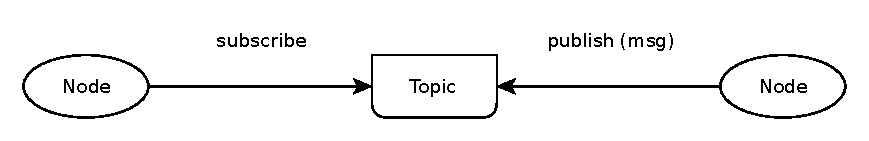
\includegraphics[width=12cm]{kapitel2/ros-topic}
  \caption{Beziehung zwischen Topics und Nodes}
  \label{Kap2:ROSTopic}
\end{figure}

Die zweite Möglichkeit ist die Kommunikation über sogenannte Services. Diese Art der Kommunikation findet nach dem Client-Server-Prinzip statt. Demnach können Nodes, wie in \autoref{Kap2:ROSService} dargestellt, Services anbieten oder diese abfragen. Es handelt sich dabei um eine "`one-to-one"'-Abfrage. Das bedeutet, dass eine Node eine Anfrage an einen Service stellt und nur diese Node antwortet. Das Nachrichtenformat ist das Format "`.srv"'. Definitionen von Services werden in der Regel im Ordner "`/msg"' definiert.

\begin{figure}[t]
  \centering
  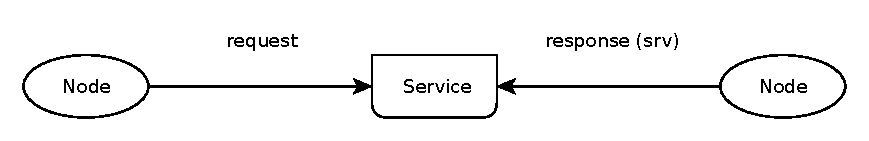
\includegraphics[width=12cm]{kapitel2/ros-service}
  \caption{Beziehung zwischen Services und Nodes}
  \label{Kap2:ROSService}
\end{figure}

Im Allgemeinen beinhaltet jede Nachricht zusätzlich zu den Daten einen sogenannten Header. Dieser enthält eine eindeutige Identifikationsnummer, einen Zeitstempel und eine Frame-ID.

Ein weiterer Bestandteil von \ac{ROS} sind die sogenannten Launch-Files. Diese sollen das Ausführen von mehreren Nodes vereinfachen, da am Ende nur noch ein einziges Launch-File gestartet werden muss. Ein Launch-File wird in XML definiert. Üblich ist es, für alle Launch-Files einen Ordner mit dem Namen "`launch"' zu erstellen. Neben dem Starten von Nodes können Launch-Files auch andere Launch-Files inkludieren. Außerdem kann eine Namensänderung von Topic-Namen definiert werden, um die Kompatibilität zwischen mehreren Packages zu gewährleisten. Dies nennt sich auch Remapping. Zuletzt bieten Launch-Files noch die Option Nodes bei Absturz neu zu starten, die Ausgabe auf dem Bilschirm auszugeben und die Option Konsolenargumente zu verarbeiten.

\lstinputlisting[language=Xml,caption={Beispiel eines Launch-Files in XML},label=lst:LaunchFileXML,float=t]{\srcloc/ROS_Launch-File.xml}

Das Launch-File in \autoref{lst:LaunchFileXML} startet zwei Nodes. Die erste Node veröffentlicht über das \ac{ROS}topic-Node die Message, welche den Befehl zum Motorstart ausführt. Die zweite Node startet die Node, welche Kommandos aufnehmen kann, um den Roboter zu bewegen. Der dritte Block startet ein externes Launch-File, welches wiederum Kommandos für einen Joystick beinhaltet, der Befehle an den p2os\_driver geben kann. Launch-Files sind hilfreich, damit alle Nodes nicht einzeln gestartet werden müssen.

Des Weiteren bietet das System mit den sogenannten Bags die Möglichkeit zum Aufzeichnen und Wiedergeben von Nachrichten bzw. spezifischer Sensordaten. Damit ist es möglich, eine Aufnahme mit der Roboter immer wieder abzuspielen, um einen Fehler zu analysieren, ohne den Roboter erneut durchlaufen lassen zu müssen. Bag-Aufnahmen oder Bag-Wiedergaben können auch in Launch-Files definiert werden. Außerdem lassen sich Aufnahmen sowohl über das Terminal als auch über eine grafische Oberfläche starten und modifizieren, wie in \autoref{Kap2:ROSBag} zu sehen ist.

\begin{figure}[t]
  \centering
  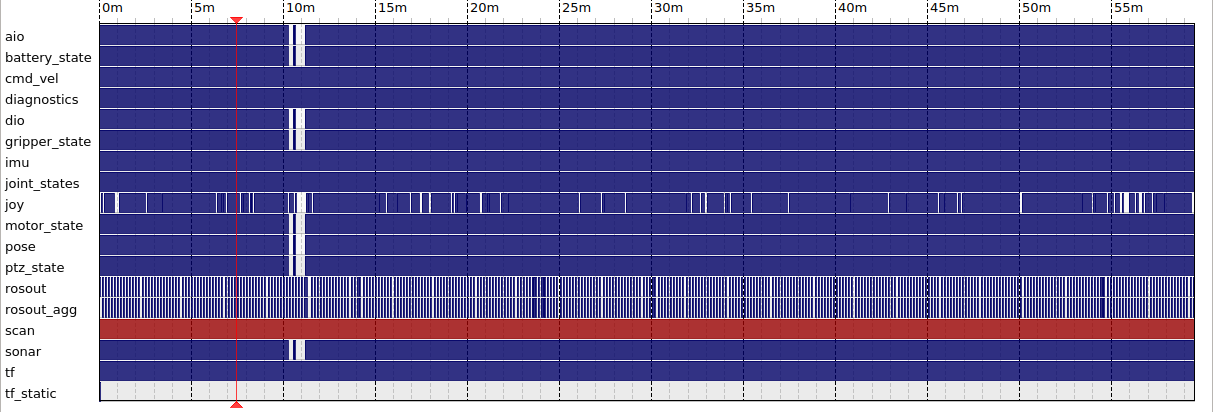
\includegraphics[width=14cm]{kapitel2/rqt-bag}
  \caption{Abspielen eines ROS-Bags mit RQT}
  \label{Kap2:ROSBag}
\end{figure}

Das Robot Operating System bietet zuletzt noch ein mächtiges Kommandozeilen-Tool, mit dem Aufgaben leichter erledigt werden können. Die in \autoref{ROS-Kommandozeile} gezeigten Kommandos, dienen als Überblick über die erläuterten Themen. \autocite{learningROSForRoboticsProgramming} \autocite{gentleIntroductionToROS}
\begin{table}[b]
  \caption{ROS-Kommandozeile}
  \label{ROS-Kommandozeile}
  \renewcommand{\arraystretch}{1.2}
  \centering
  \sffamily
  \begin{footnotesize}
    \begin{tabular}{l l}
    \toprule
    \textbf{Kommando} & \textbf{Erklärung}\\
    \midrule
    \multicolumn{2}{c}{\textit{Allgemein}}\\
    roscore & Startet den ROS-Master\\
    rospack list & Gibt alle Packages aus\\
    roscd package-name & Wechselt das Verzeichnis zu einem Package\\
    rosls & Zeigt die Inhalte eines Packages an\\
    rospack find package-name & Findet das Verzeichnis eines Packages\\
    \multicolumn{2}{l}{}\\
    \multicolumn{2}{c}{\textit{Nodes}}\\
    rosrun package-name exec-name & Startet eine Node eines Packages\\
    rosnode list & Listet alle Nodes auf\\
    rosnode info node-name & Gibt Informationen zu einer Node aus\\
    rosnode kill node-name & Beendet eine Node\\
    \multicolumn{2}{l}{}\\
    \multicolumn{2}{c}{\textit{Topics}}\\
    rostopic list & Listet alle Topics auf\\
    rostopic echo topic-name & Gibt die Inhalte eines Topics aus\\
    rostopic info topic-name & Gibt Informationen zu einem Topic aus\\
    rosmsg show message-type-name & Zeigt den Aufbau der Message an\\
    \multicolumn{2}{l}{}\\
    \multicolumn{2}{c}{\textit{Services}}\\
    rosservice list & Listet alle Services auf\\
    rosservice node service-name & Gibt die Node aus, die den Service anbietet\\
    rosservice info service-name & Gibt Informationen zu einem Service aus\\
    rossrv show service-data-type-name & Zeigt den Aufbau der Service-Message an\\
    \multicolumn{2}{l}{}\\
    \multicolumn{2}{c}{\textit{Launch-Files}}\\
    roslaunch filename & Führt das Launch-File aus\\
    \multicolumn{2}{l}{}\\
    \multicolumn{2}{c}{\textit{Bags}}\\
    rosbag record -a & Zeichnet alle Topics auf\\
    rosbag play filename & Spielt das ROS-Bag wieder ab\\
    rosbag info filename & Gibt Informationen zu einem ROS-Bag aus\\
    \bottomrule
    \end{tabular}
  \end{footnotesize}
  \rmfamily
\end{table}

\section{Pioneer 3-DX}

Im nächsten Schritt wird der zu verwendende Roboter für die Kartierung vorgestellt und dargelegt, wie dieser mit dem Robot Operating System interagiert.

Der Pioneer 3-DX ist ein mobiler Roboter, der in verschiedenen Bereichen der Robotik eingesetzt werden kann, da er beliebig erweiterbar ist. Beispielsweise lässt dieser sich für die Kartierung einsetzen, wenn er um einen Laserscanner erweitert würde. Eine weitere Möglichkeit ist, dass der Roboter alltägliche Aufgaben erfüllen kann, in dem man ihn mit einem Greifarm ausstattet.

Das Modell 3-DX an sich ist 44,5 cm lang, 39,3 cm breit und 23,7 cm hoch, wiegt 9 Kilogramm und kann maximal 25kg tragen. Des Weiteren besteht der Roboter aus zwei Rädern und einem zusätzlichen Stützrad. Die Art des Fahrens ist das sogenannte Differential Drive. Außerdem besitzt der Pioneer 3-DX Ultraschallsensoren sowie Stoßfänger, falls alle anderen Mechanismen zur Verhinderung eines Aufpralls nicht greifen. \autocite{pioneer3operationsmanual}

Für diese Arbeit ist ein Umbau des Pioneer 3-DX eingesetzt worden. Zusätzlich zu den genannten Bauteilen kommt noch ein Computer, ein Laserscanner sowie eine Intertial Measurement Unit (IMU) zum Einsatz. Beim Computer handelt es sich um die Linux Distribution Ubuntu 18.04.2 LTS. Dieser ist auf der Roboter-Basis angebracht. Der Computer hat 4 GB Arbeitsspeicher sowie 2 GB an zusätzlichem SWAP. Der Laserscanner ist der SICK LMS, der ebenfalls auf der Roboter-Basis angebracht ist. Die IMU ist die Tinkerforge Brick 2.0.

\begin{figure}[t]
  \centering
  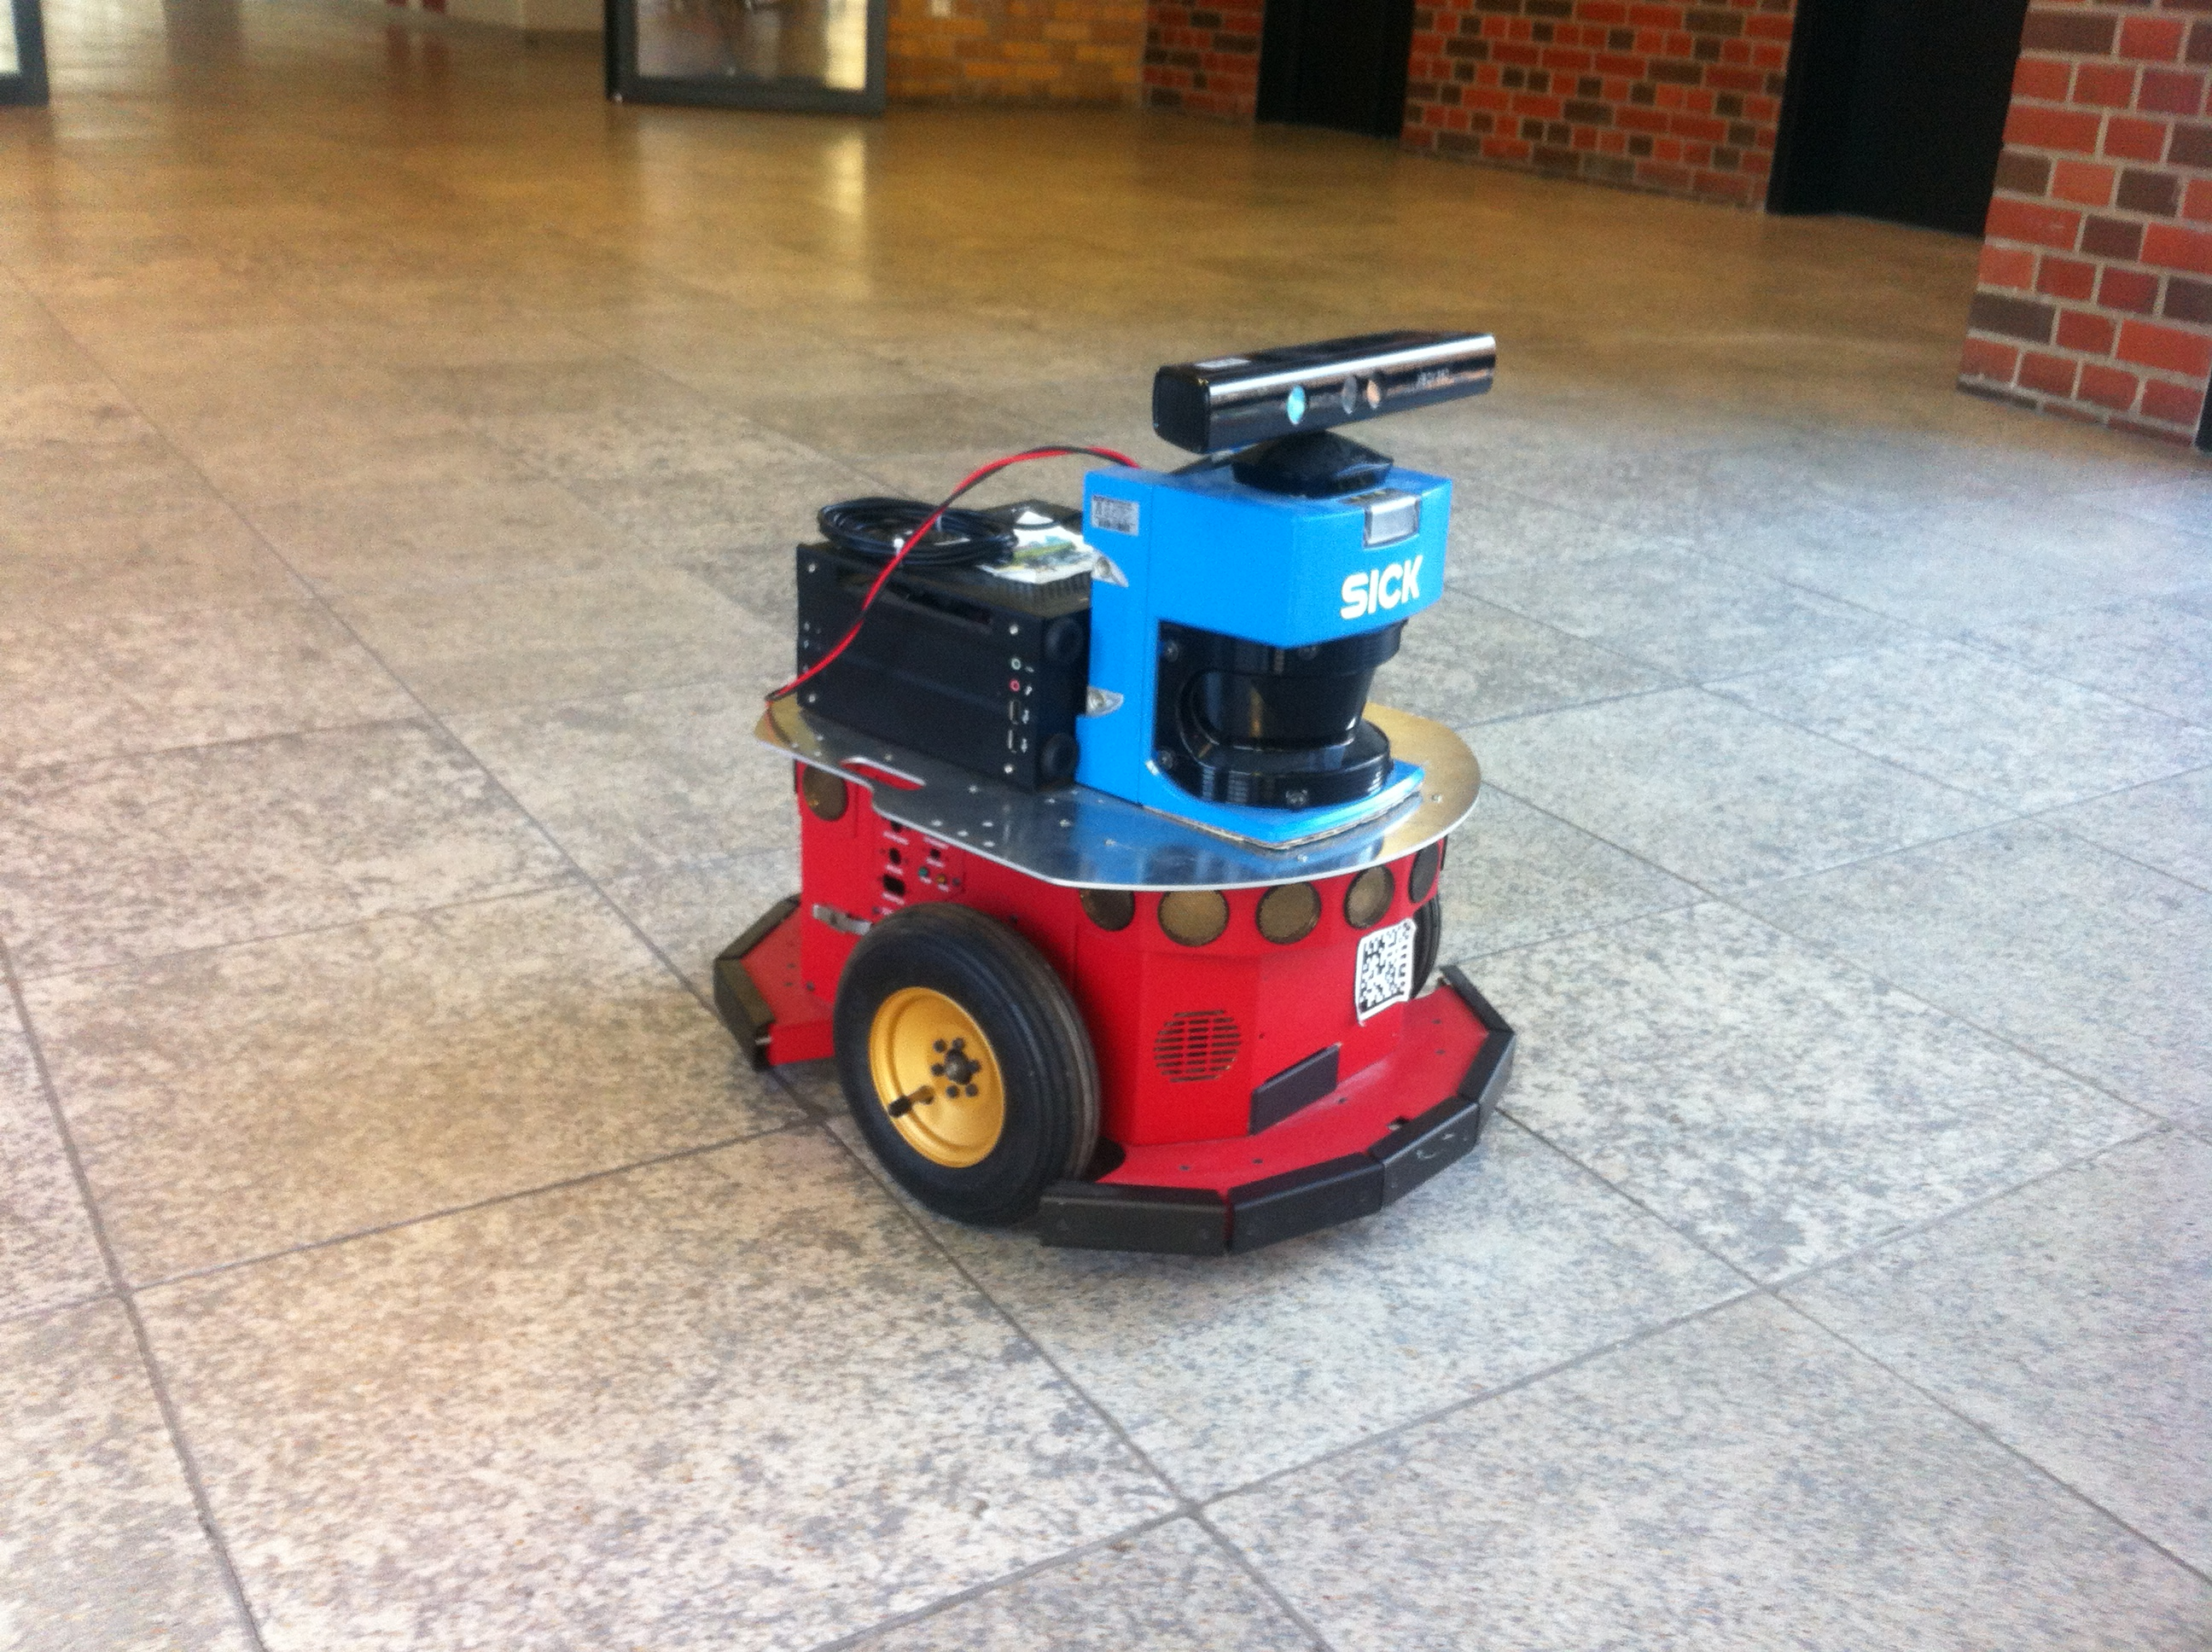
\includegraphics[width=10cm]{kapitel2/pioneer-umbau}
  \caption{Pioneer 3-DX mit Lasercanner, Kinect und Computer}
  \label{Kap2:Pioneer3DX}
\end{figure}

Der Pioneer 3-DX lässt sich im Netzbetrieb oder im Akkubetrieb starten. Dabei sollte mindestens eine Spannung von 12 Volt anliegen. Der Roboter besitzt drei Plätze für Akkus, die gleichzeitig genutzt werden können. \autocite{pioneer3operationsmanual}